\documentclass[oneside]{book}

%% 必须的包
\usepackage{bm}
\usepackage{amsmath}
\usepackage{amsfonts}
\usepackage{amssymb}
%\usepackage{mathtools}
\usepackage{xcolor}
\usepackage{siunitx}
\usepackage{booktabs}
\usepackage{graphicx}
\graphicspath{{fig/}}
\DeclareGraphicsExtensions{.pdf,.eps,.png,.jpg,.jpeg,.bmp}

%% 中文文字处理
\colorlet{title}{blue!40!black}
\usepackage[heading = true]{ctex}
    \ctexset{today = old}
    \pagestyle{plain}  % 自定义板式
    %% 标题设置
    \ctexset{
        chapter = {
            format += \color{title},
            pagestyle = chapterpage,
        },
        section = {
            format = \bf\raggedright\color{title}\zihao{4},
            numberformat = \rmfamily,
        },
        subsection = {
            format = \rmfamily\heiti\raggedright\color{title}\zihao{5},
        },
    }%

% 问题环境
\newtheorem{prob}{问题}[chapter]
\renewcommand{\theprob}{\arabic{prob}}

%% 字体设置
\usepackage{fontspec}
    \setmainfont{Adobe Garamond Pro}  % TeX Gyre Pagella
    \setsansfont{Arial}
    \setmonofont{Iosevka Type Slab}  % Source Code Pro, Consolas, DejaVu Sans Mono
    \setCJKmainfont[BoldFont={Source Han Sans SC}, ItalicFont={KaiTi}]{Source Han Serif SC}
    \setCJKmonofont{Sarasa Term SC}  % FangSong
    \setCJKsansfont{Source Han Sans SC}

\usepackage{geometry}
    \geometry{paper=a4paper,
%        hmargin = 2cm,
        vmargin = 3cm,
    }%

%% 页眉页脚
\usepackage{fancyhdr}
\pagestyle{fancy}
    \fancyhead{}
        \lhead{\kaishu\nouppercase{\leftmark}}
        \rhead{\thepage}
    \fancyfoot{}
% 章标题所在页专用版式
\fancypagestyle{chapterpage}{%
    \chead{\slshape\leftmark}
    \lhead{\sffamily 传递现象与热力学笔记}
    \rhead{\thepage}
}

\usepackage{enumitem}%列表
\setlist[description]{%
    font=\bfseries\color{blue!40!black},
    noitemsep,
    nosep,
    align=left,
    leftmargin=!,
    labelindent=\parindent,
    labelwidth=20mm,
    labelsep=1em,
    itemindent=0mm,
}
\setlist[enumerate]{%
    noitemsep,
    nosep,
    leftmargin=0pt,
    itemindent=*,
    labelindent=\parindent,
    listparindent=\parindent,
}
\setlist[itemize]{%
    nosep,
    leftmargin=\parindent,
}

%===========================图表标题样式============================
\usepackage[hypcap=true,hypcapspace=1cm]{caption}
\captionsetup[figure]{%
    labelsep=quad,
    justification=centering,
    labelfont=bf,
    textfont={sf,color=title},
}%
\captionsetup[table]{%
    labelsep=quad,
    justification=centering,
    labelfont=bf,
    textfont={sf,color=title},
}%

%% 参考文献
\usepackage[
    backend=biber,
    bibstyle=gb7714-2015,
    citestyle=gb7714-2015,
    ]{biblatex}
%biblatex宏包的参考文献数据源加载方式
\addbibresource[location=local]{ref.bib}

%% 超链接
\usepackage{hyperref}
    \hypersetup{%
        bookmarksopen=true,  % 展开书签
        bookmarksnumbered=true,  % 显示书签编号
        bookmarksopenlevel=1,
        unicode=true,  % 使书签支持unicode字符
        %链接、颜色
        breaklinks=true,  % 链接自动换行
        colorlinks=true,  % 加颜色区分链接
        linkcolor=title,
        citecolor=black,  % 文献序号颜色
    }
    %定制pdf属性
    \hypersetup{%
        pdftitle={transport phenomena and thermodynamics},
        pdfauthor={邹思宇},
        pdfkeywords={transport phenomena and thermodynamics},
        pdfstartview=Fit,%整个页面适合窗口
        pdfcreator={XeLaTeX \& TeXStudio \& MiKTeX}
    }%

%自动引用
\AtBeginDocument{%
    \def\figureautorefname{图}%
    \def\tableautorefname{表}%
    \def\partautorefname{卷}%
    \def\appendixautorefname{附录}%
    \def\equationautorefname{式}%
    \def\Itemautorefname{列表}%
    \def\chapterautorefname{章}%
    \def\sectionautorefname{节}%
    \def\subsectionautorefname{小节}%
    \def\subsubsectionautorefname{条目}%
    \def\paragraphautorefname{自然段}%
    \def\Hfootnoteautorefname{脚注}%
    \def\AMSautorefname{式}%
    \def\theoremautorefname{定理}%
    \def\pageautorefname{页}%
}%

%% url样式
\newfontfamily\urlfont{PT Sans Narrow}
\def\UrlFont{\urlfont}
\urlstyle{urlfont}

\begin{document}
    \frontmatter
    \tableofcontents
    \mainmatter
    \chapter{Momentum Transport}

\section{基本数学知识}
\subsection{大学白学了}

\[\frac{d}{dx}(uv) = u\frac{dv}{dx} + v\frac{du}{dx}\]

\subsection{矢量计算}

几个基本的等式:

\[\nabla s = \frac{\partial s}{\partial x}\bm{i} +  \frac{\partial s}{\partial y}\bm{j} + \frac{\partial s}{\partial z}\bm{k}\]

\[\nabla\cdot\bm{u} = \frac{\partial u}{\partial x} + \frac{\partial v}{\partial y} + \frac{\partial w}{\partial z}\]

\[\nabla^2\bm{u} = \frac{\partial^2 u}{\partial x^2} + \frac{\partial^2 v}{\partial y^2} + \frac{\partial^2 w}{\partial z^2} \]

\[\nabla\cdot (s\mathbf{u}) = s\nabla\cdot\bm{u}+\bm{u}\cdot\nabla s\]

\subsection{Gauss散度定理}
整个控制体内的源汇项=控制体表面的净通量:

\begin{equation}\label{Gauss}
\int_{V}(\nabla\cdot \bm{u})dV = \int_{S} (\bm{u\cdot n})dS
\end{equation}

\subsection{Leibniz积分法则}

给出了一个对积分变量为函数的积分求导的法则,右侧第一项解释了积分随时间的变化,二三两项区域内物理量的得失。

\begin{equation}
    \frac{d}{dt} \int_{a(t)}^{b(t)} \phi(x,t) dx = \int_{a(t)}^{b(t)} \frac{\partial \phi}{\partial t} dx + \phi(b(t),t) \frac{\partial b}{\partial t} - \phi(a(t),t)\frac{\partial a}{\partial t}
\end{equation}

对由面$ S(t) $包围的封闭三维空间$ V(t) $来讲,假设面的移动速度为$ \mathbf{v_s} $,有如下积分法则:

\begin{equation}
    \frac{d}{dt} \int_{V(t)} \phi dV = \int_{V(t)} \frac{\partial \phi}{\partial t} dV + \int_{S(t)} \phi(\mathbf{v_s}\cdot \mathbf{n}) dS
\end{equation}

若控制体不移动,则:

\begin{equation}\label{Leibniz}
\frac{d}{dt} \int_{V(t)} \phi dV = \int_{V(t)} \frac{\partial \phi}{\partial t} dV
\end{equation}


\section{无量纲数}\label{dimensionless-number}

Reynolds Number,定义为惯性力和粘性力的比:

\[ Re = \frac{\rho UL}{\mu} \]

Grashof Number,定义为浮力和粘性力的比,$ \nu $为动力粘度:

\[ Gr = \frac{g\beta\Delta TL^3}{\nu^2} \]

P\'{e}clet Number,定义为对流传递速率与扩散传递速率之比,$ D $为质量扩散系数:

\[ Pe =
\begin{cases}
\frac{\rho ULc_p}{k} = \frac{UL}{\alpha} = RePr & \text{for heat transfer}\\
\frac{UL}{D} = ReSc & \text{for mass transfer}
\end{cases}
\]

Prandtl Number,定义为动量扩散率和热扩散率之比(也代表流动边界层和热边界层之比),$ k $为导热系数,$ \alpha $为热扩散系数,$ \nu $为动力粘度($ \nu = \mu/\rho $)。$ Pr<1 $时,热边界层比速度边界层厚;$ Pr>1 $,热边界层比速度边界层薄。

\[ Pr = \frac{\mu c_p}{k} = \frac{\mu/\rho}{k/\rho c_p} = \frac{\nu}{\alpha} \]

Schmidt Number,定义为动量扩散率和质量扩散率之比,用于描述同时存在动量和质量扩散过程的流体流动。$ Sc $在质量传递中的作用与$ Pr $在能量传递中的作用类似,物理意义上表示速度边界层与传质边界层的相对厚度。$ Sc<1 $时,传质边界层比速度边界层厚;$ Sc>1 $时,传质边界层比速度边界层薄。

\[ Sc = \frac{\nu}{D} \]

Lewis Number,定义为热扩散系数与质量扩散系数之比,系统涉及到质量和能量的同时传递:

\[Le = \frac{\alpha}{D}\]

Nusselt Number,定义为对流和热传导之比:

\[Nu = \frac{hL}{k}\]

Sherwood number,定义为分子质量传递阻力与对流质量传递阻力之比,其中$ h $为对流传质系数(\si{\meter\per\second}):

\[Sh = \frac{hL}{D}\]

Mach Number,定义为速度和介质中声速之比:

\[ M = \frac{|\mathbf{v}|}{a} \]

声速由下式计算,其中$ \gamma=c_p/c_v $为比气体常数:

\[a=\sqrt{\gamma\left( \frac{\partial p}{\partial \rho} \right)_T}\]

对理想气体而言,简化如下:

\[a=\sqrt{\gamma RT}\]

Eckert Number,动能和焓之比。如果$ Ec\ll 1 $,能量方程中的粘性耗散和压力功就可以忽略(事实上这个无量纲数就是为了表明,在速度不太高的情况下,可压缩流体的的粘性耗散和压力功可以忽略):

\[Ec=\frac{\mathbf{v\cdot v}}{c_p\Delta T}\]

Froude number,定义为特征速度和重力波速度之比,用来表征固体在流体中运动的情况,$ Fr $越高意味着固体所受阻力越大:

\[Fr = \frac{U}{\sqrt{gL}}\]

Weber Number,定义为惯性力和表面张力之比:

\[We=\frac{\rho U^2 L}{\sigma}\]

\section{常见物理量}

动力粘度$ \mu $,单位\si{\pascal\per\second}或\si{\kilogram\per\meter\per\second},定义为剪应力与剪切速率之比。

\[\tau = \mu\frac{\partial u}{\partial y}\]

运动粘度,单位\si{\meter\squared\per\second},定义为粘度与密度的比值。

\[\nu=\frac{\mu}{\rho} \] 

\section{Euler和Lagrange参考系}

经典力学认为孤立系统的物理量是守恒的,对于流体系统,典型的守恒定律包括质量、动量和能量守恒。涉及流体流动和传递现象的守恒定律在数学上分两类描述,Lagrange方法(material volume)和Euler方法(control volume)。

Lagrange方法跟踪每个流体微团的空间位置随时间的变化,微团的物理量表示为流体质点和时间的函数。初始时刻$ t_0 $时流体质点位于$ \bm{r}_0(x_0, y_0, z_0) $,相应的物理量表示为$ \phi(\bm{r}_0, t) $,不同的$ \bm{r}_0 $代表不同的流体微团。固定$ \bm{r}_0 $而让时间$ t $变化,得到的是某一确定的微团的空间位置及其相关物理量随时间的变化;反之,固定时间$ 
t $而让$ \bm{r}_0 $变化,将得到同一时刻下不同流体微团的空间位置及其相关物理量随时间的变化。

\begin{equation}
\phi = \phi(\bm{r}_0, t)
\end{equation}

Euler方法将流体微团的运动和物理量变化表示为固定的空间点$ \bm{r}_0(x, y, z) $和时间$ t $的函数。固定空间点$ \bm{r} $而让时间$ t $变化,得到某一空间点上物理量随时间的变化规律;反之,固定时间$ t $而让空间点$ \bm{r} $变化,将得到某一时刻物理量的空间分布。

\begin{equation}
\phi = \phi(\bm{r}, t)
\end{equation}

Lagrange参考系下,流体微团的速度可表示为:

\[ \bm{u}(\bm{r}_0, t) = \frac{\partial \bm{u}(\bm{r}_0)}{\partial t} \]

代入Euler参考系,得到两种参考系的关联:

\begin{equation}
\bm{u}(\bm{u}(\bm{r}_0, t), t) = \frac{\partial \bm{u}(\bm{r}_0)}{\partial t}
\end{equation}

基于这两种描述,可以在流体粒子穿过空间的固定点(Euler方法)或沿着流体微团的运动路径(Lagrange方法)来跟踪流体微团的运动以测量流体性质变化。

\section{随体导数}

场变量$ \phi(\bm{r}, t) $既可以是一个标量($ \rho, T $),也可以是一个矢量($ \bm{u} $)。Euler描述下,场变量的导数$ \partial\phi/\partial t $是某一固定空间点上场变量$ \phi $对时间的变化率;而与流体微团相关的物理量随时间的变化率$ D\phi/Dt $称为随体导数或物质导数(substantial or material derivative)。微元中的物理量$ \phi $是位置和时间的函数,随体导数$ D\phi/Dt $定义为:

\begin{align}
\frac{D\phi}{Dt} & = \frac{\partial \phi}{\partial t}+\frac{\partial \phi}{\partial x}\frac{dx}{dt} + \frac{\partial \phi}{\partial y}\frac{dy}{dt} + \frac{\partial \phi}{\partial z}\frac{dz}{dt} \\
& =\frac{\partial \phi}{\partial t}+u\frac{\partial \phi}{\partial x}+v\frac{\partial \phi}{\partial y}+w\frac{\partial \phi}{\partial z} \\
& = \underbrace{\frac{\partial \phi}{\partial t}}_{\text{local rate
    of change}}+\underbrace{\bm{u}\cdot \nabla \phi}_{\text{convective rate
    of change}}
\end{align}

\section{Reynolds输送定理}

\textbf{物质导数}给出了与流体质点相关的物理量随时间的变化率,是观察者随同流体质点一起运动所观察到的场变量$ \phi $的变化率。为了在Euler参考系下描述这种守恒定律,需要知道等效的物质积分的变化率,Reynolds输送定理提供了在Eulerian参考系下计算有限大小物质体的物理量随时间的变化率的方法。

使用$ \phi $来代表流体的任意性质(质量、动量、能量等),物质体积(material volume,MV)内的物理量$ \phi $的瞬时变化等于控制体积(control volume,CV)内的物理量的瞬时变化加上进出控制体控制面(control surface,S)的物理量的净流量。

\begin{equation}
\left( \frac{d\phi}{dt} \right)_{MV} = \int_V \frac{\partial\phi}{\partial t}dV + \int_S \phi\mathbf{v\cdot n} dS
\end{equation}

运用Gauss散度定理(\autoref{Gauss})将面积分转换为体积分:

\begin{equation}
\left( \frac{d\phi}{dt} \right)_{MV} = \int_V \left[ \frac{\partial\phi}{\partial t} + \nabla\cdot(\phi\mathbf{v}) \right]dV
\end{equation}

配合随体导数和矢量计算可写成:

\begin{equation}\label{Reynolds_transport_theorem}
\left( \frac{d\phi}{dt} \right)_{MV} = \int_V \left[ \frac{D\phi}{Dt} + \phi\nabla\cdot\mathbf{v} \right]dV
\end{equation}

\autoref{Reynolds_transport_theorem}称为Reynolds输送定理,可以用来推导空间点固定的Euler形式的守恒定律。

\section{质量守恒/连续性方程}

质量守恒定律指出,在没有质量源和汇的情况下,区域质量守恒。在Lagrangian参考系的物质坐标下,质量守恒定律写作:

\begin{equation}
\left(\frac{dm}{dt}\right)_{MV} = 0
\end{equation}

根据\autoref{Reynolds_transport_theorem}的Reynolds输送定理,Euler参考系下的质量守恒定律写作:

\begin{equation}
\int_V \left[\frac{D\rho}{Dt} + \rho\nabla\cdot\mathbf{v} \right]dV = 0
\end{equation}

对任意控制体运用Euler参考系下的守恒定律,积分为0导出微分形式的质量守恒方程:

\begin{gather}
\frac{D\rho}{Dt} + \rho\nabla\cdot\mathbf{v} = 0 \\
\frac{\rho}{t} + \nabla\cdot(\rho\bm{u}) = 0
\end{gather}

对不可压缩流体来说,密度$ \rho $视为常数,质量守恒方程为:

\begin{equation}
\nabla\cdot\bm{u} = 0
\end{equation}

\section{动量守恒}

守恒形式在\textbf{空间固定的控制体}(控制体位置、形状不变)上推导而来,所有变量全部写在偏导符号内;非守恒形式在\textbf{运动的控制体}(永远由相同的流体微团构成)上推导而来,部分流场变量在偏导外。使用守恒型的原因有两个:1. 程序和算法设计方便,守恒形式可以写成统一的格式;2. 数值计算上能减少误差,守恒型方程在流场有间断时(比如接触间断、激波之类),能得到平滑的解而非守恒型则容易产生震荡。守恒型方程的守恒变量在跨过激波时要么很小要么为零,所以能提高激波数值解的质量。

总的来说,守恒形式和非守恒形式在数学上是等价的。FVM是基于守恒形式的。

\subsection{Non-Conservative Form}
由随体导数的Reynolds输送定理可推导出:

\begin{equation}
\int_{V}\left[ \frac{D}{Dt}(\rho\bm{u}) + (\rho\bm{u}\nabla\cdot \bm{u}) - \bm{f} \right]dV = 0
\end{equation}

即:

\begin{equation}
\frac{D}{Dt}(\rho\bm{u}) + (\rho\bm{u}\nabla\cdot \bm{u}) = \bm{f}
\end{equation}

用微积分基本定理拆开,发现2、3两相就是连续性方程(不信自己拆),等于0:

\begin{equation}
\rho\frac{D\bm{u}}{Dt}(\rho\bm{u}) + \underbrace{ \bm{u}\frac{D\rho}{Dt} + \rho\nabla\cdot\bm{u} } = \bm{f}
\end{equation}

然后得到非守恒形式的动量方程,其中$ \bm{f} $为各种力:

\begin{equation}
\rho\left[ \frac{\partial \bm{u}}{\partial t} + \bm{u}\cdot\nabla\bm{u} \right] = \bm{f}
\end{equation}

\subsection{Conservative Form}
用那个Gauss散度定理推出的Reynolds输送定理可推导出:

\begin{equation}
\int_{V}\left[ \frac{\partial(\rho\bm{u})}{\partial t} + \nabla\cdot(\rho\bm{uu}) - \bm{f} \right]dV = 0
\end{equation}

即:

\begin{equation}
\frac{\partial(\rho\bm{u})}{\partial t} + \nabla\cdot(\rho\bm{uu}) = \bm{f}
\end{equation}

写成常见的守恒形式,左边的为各种力$ \bm{f} $,其中$ \tau $为应力张量,$ F $为体积力:

\begin{equation}
\frac{\partial \rho\bm{u}}{\partial t} + \nabla\cdot(\rho\bm{uu}) = -\nabla\cdot p\bm{I} + \nabla\cdot\tau + F
\end{equation}

只需要把体积力和压力梯度项看成源项,动量方程就能看成是对流扩散方程。动量的扩散对应的是流体的粘性耗散,质量扩散,温度扩散,动量扩散,这几种扩散从数学方程上看是非常相似的,因为他们都和分子无规则运动相关,分子的无规则运动能够将流体空间位置上物理量分布不均扯平,这几种扩散作用的基本物理过程,都可以用统计热力学进行分析。

\section{应力张量}
动量方程中主要包括两种力,表面力(压力、粘性力)和体积力(重力等)。

\subsection{Surface Forces}
主要是压力和粘性剪应力。压力为正应力$ \tau_{ii} $,使有限控制体体积发生变化;粘性剪应力为切应力$ \tau_{ij} $,使有限控制体形状发生改变,但是体积不变;

故,应力张量可分为两个部分:

\[-p\bm{I}+\tau\]

\subsection{Body Forces}

重力:

\[\bm{f}_b = \rho \bm{g}\]

由旋转引起的Coriolis forces和Centrifugal forces

\section{牛顿流体的应力张量和动量方程}
对牛顿流体来讲,应力张量是剪应力的线性函数。

\begin{equation}
\tau = \mu\left(\nabla\bm{u}+(\nabla\bm{u})^T\right)+\lambda(\nabla\cdot \bm{u})\bm{I}
\end{equation}

对不可压流体来说$ \nabla\cdot\bm{u} = 0 $,动量方程的一般为:

\begin{equation}
\frac{\partial \rho\bm{u}}{\partial t} + \nabla\cdot(\rho\bm{uu}) = -\nabla p\bm{I} + \nabla\cdot(\mu\left(\nabla\bm{u}+(\nabla\bm{u})^T\right)) + F
\end{equation}

如果粘度为常数(一般等温会出现这种情况),动量守恒可进一步简化。无粘流体直接去掉粘度了事:

\begin{equation}
\frac{\partial \rho\bm{u}}{\partial t} + \nabla\cdot(\rho\bm{uu}) = -\nabla p\bm{I} + \mu\nabla^2\bm{u} + F
\end{equation}

\section{通用的守恒方程}
增加率+净流出=扩散增加率+源项

\begin{equation}
\underbrace{\frac{\partial (\rho\phi)}{\partial t}}_{\text{unsteady term}} +
\underbrace{\nabla\cdot(\rho\phi\bm{u})}_{\text{convection term}} =
\underbrace{\nabla(\Gamma\nabla\phi)}_{\text{diffusion term}} +
\underbrace{S}_{\text{source term}}
\end{equation}

在有限体积法中,会在整个控制体内对方程积分:

\begin{equation}
\int_{CV}\frac{\partial (\rho\phi)}{\partial t}dV + \int_{CV}\nabla\cdot(\rho\phi\bm{u})dV = \int_{CV}\nabla\cdot(\Gamma\nabla\phi)dV + \int_{CV}SdV
\end{equation}

然后用Gauss散度定理将对流-扩散项从体积分改为面积分,同时用\autoref{Leibniz}所示的Leibniz积分法则改写第一项。

\begin{equation}
\frac{\partial}{\partial t}\left(\int_{CV}\rho\phi dV\right) + \int_{A}\bm{n}\cdot(\rho\phi\bm{u})dV = \int_{A}\bm{n}\cdot(\Gamma\nabla\phi)dV + \int_{CV}SdV
\end{equation}

有限体积法的积分方程具有非常自然的物理意义,左边第一项表示物理量$ \phi $在控制体中的变化率,左边第二项表示控制体面上的净流出量(即对流项),右边第一项表示扩散引起的增量,最后一项为源-汇项。

对于稳态问题,时间导数为0:

\begin{equation}
\int_{A}\bm{n}\cdot(\rho\phi\bm{u})dV = \int_{A}\bm{n}\cdot(\Gamma\nabla\phi)dV + \int_{CV}SdV
\end{equation}

对瞬态问题,需要在每一个时间步内进行积分:

\begin{equation}
\int_{\Delta t}\frac{\partial}{\partial t}\left(\int_{CV}\rho\phi dV\right) + \int_{\Delta t}\int_{A}\bm{n}\cdot(\rho\phi\bm{u})dV = \int_{\Delta t}\int_{A}\bm{n}\cdot(\Gamma\nabla\phi)dV + \int_{\Delta t}\int_{CV}SdV
\end{equation}

\section{FVM 有限体积法}

基本思路:

\begin{enumerate}
    \item 将计算区域划分为一系列不重复的控制体积 ,每一个控制体积都有一个节点作代表 ,将待求的守恒型微分方程在任一控制体积及一定时间间隔内对空间与时间作积分 ;
    \item 对待求函数及其导数对时间及空间的变化型线或插值方式作出假设 ;
    \item 按选定的型线作出积分并整理成一组关于节点上未知量的离散的代数方程,使用代数方法求解。
\end{enumerate}

\subsection{对流-扩散问题的离散方式}

\begin{description}
    \item[一阶迎风] 一阶精度,绝对稳定,假设界面上的物理量和上游的物理量一样。可以获得物理上能接受的解,但当$ Pe $数较大时,假扩散比较严重,需要加密网格;
    \item[二阶迎风] 二阶精度,绝对稳定,边界上的物理量由上游的两个点插值得出。通用存在假扩散;
    \item[QUICK] 其对流项有三阶精度(用了三个数据点插值),扩散项仅有二阶精度(通常等于中心差分);需要使用结构化网格(六面体或四面体网格)才能发挥高阶精度的优势。
\end{description}

\subsection{压力速度耦合}

\begin{description}
    \item[SIMPLE] robust,一般只用于求解不可压缩流动,需要先假定一个压力,然后计算速度,最后循环修正压力和速度直至收敛;
    \item[SIMPLEC] SIMPLE的改进算法,能更快的收敛;
    \item[PISO] 常用于瞬态计算,对瞬态计算效率较高
\end{description}

\section{自然对流 natural convection}

自然对流由浮力引起,密度差越大,浮力越大。

在强制对流里面,使用$Re$数来描述流动行为,其表示惯性力(the inertial
forces)与粘性力(the viscous forces)之比。对于内部驱动的流动行为——比如自然对流,初始速度未知,无法使用$Re$数表征流动行为。通常用The Grashof number来描述自然对流,其表示流体\textbf{浮力与粘性力的比值}(It describes the ratio of the time scales for viscous diffusion in the fluid and the internal driving force (the buoyancy force).)。当$Gr>10^9$时,自然对流转变为湍流。

%对湿空气来讲,密度依赖于温度和含水率,$Gr$数定义如下:
%\begin{equation}
%    Gr = \frac{g\rho (\rho_{ext} - \rho_s) L^3}{\mu^2}
%\end{equation}
%
%$\rho_s$代表热表面的密度(solid),$\rho_{ext}$代表the free stream density,$\rho$代表流体密度。

$Gr$数定义如下:

\begin{equation}
Gr = \frac{g\beta (T_s - T_\infty)L^3}{(\mu/\rho)^2} = \frac{g\beta\Delta T L^3}{\nu^2}
\end{equation}

通常,$ T_s $为表面温度,$ T_\infty $为远离表面的温度,$ L $为特征长度,$\mu/\rho=\nu$,定义为动力粘度。

对于垂直平板而言,特征长度为板高;水平平板特征长度为表面积除以周长,$ A/P $;垂直圆管特征长度为管长;水平圆管特征长度为管径$ D $;球的特征长度为直径$ D $。详情参见文献\footnote{Cengel Y. Heat and mass transfer: fundamentals and applications[M]. McGraw-Hill Higher Education, 2014. p542}。

$\beta$为热膨胀系数(the coefficient of thermal expansion),定义为:
\begin{equation}
    \beta = -\frac{1}{\rho} \left( \frac{\partial \rho}{\partial T} \right)_T
\end{equation}

对理想气体而言,$\beta$简化为:
\begin{equation}
    \beta = \frac{1}{T}
\end{equation}

同样,The Rayleigh number也可以用来表征自然对流,$Ra$数定义如下:
\begin{equation}
    Ra = GrPr =\frac{g\beta\rho^2 C_p |T-T_{ext}|L^3}{k\mu}
\end{equation}

其中,$Pr$为The Prandtl number,定义如下。如果$ Pr<1 $,则粘性力对浮力没有显著的影响。

\begin{equation}
    Pr = \frac{\nu}{\alpha} = \frac{c_p\mu}{k}
\end{equation}

$\alpha$为热扩散系数,定义为:
\begin{equation}
    \alpha = \frac{k}{\rho c_p}
\end{equation}

%若密度仅仅依赖于温度,$Ra$数定义如下:
%\begin{equation}
%    Ra = \frac{g\rho C_p |\rho_{ext}-\rho_s|L^3}{k\mu}
%\end{equation}

如果使用无量纲数判断自然对流属于层流,则可以使用下式估算自然对流的速度:

\begin{equation}
U_0 =\sqrt{g\alpha\Delta T L}
\end{equation}

\subsection{自然对流与强制对流的相对大小}

Ref: Heat and Mass Transfer:Fundamentals and Applications(p540)

两者的相对大小通过$ Gr/Re^2 $来表征。如果$ Gr/Re^2 \gg 1 $,惯性力可以忽略不计,自然对流效应占主导地位;如果$ Gr/Re^2 \ll 1 $,浮力可以忽略不计,必须考虑强制对流;如果$ Gr\approx Re^2 $,惯性力和浮力同时存在,必须同时考虑自然对流和强迫对流的影响,在这种情况下,这种流动被称为混合对流。

\section{真空系统}
真空系统的气体流动需要使用与传统流体流动问题不同的物理方程来描述。在低压环境下,气体分子的平均自由程与系统的尺度相当,气体的稀薄效应变得很重要。通常情况下,稀薄度可以通过克努森数\footnote{\url{https://en.wikipedia.org/wiki/Knudsen_number}}来描述,分辨真空系统中是使用统计力学还是连续介质假设来描述流体流动。

\begin{equation}\label{Knudsen}
Kn = \frac{\lambda}{L}
\end{equation}

其中$ \lambda $为是气体分子的平均自由程,$ L $为系统的特征尺寸。在动力学理论(kinetic theory)中,分子的平均自由程\footnote{\url{https://en.wikipedia.org/wiki/Mean_free_path}}指分子在与其他分子碰撞之间行进的距离,其中$ k_B $为玻尔兹曼常数,$ d $为分子直径。

\begin{equation}
\lambda = \frac{k_B T}{\sqrt{2}\pi d^2 p}
\end{equation}

\autoref{knudsenVSflow}显示了不同$ Kn $数下的流型及系统适用的控制方程。

\begin{table}[h]
    \centering
    \caption{Knudsen数与流体流动类型}
    \label{knudsenVSflow}
    \begin{tabular}{cc}
        \toprule
        $ Kn $数 & 流动类型 \\
        \midrule
        $ Kn<0.01 $ & 连续介质假设,使用Navier-Stokes方程和传统的计算流体力学方法 \\
        $ 0.01<Kn<0.1 $ & 滑移流,Navier-Stokes方程,壁面处使用\textbf{滑移边界条件}来模拟\textbf{克努森层} \\
        $ 0.1<Kn<10 $ & 过渡流,大部分流体区域都属于克努森层,必须使用稀薄气体动力学方法 \\
        $ Kn>10 $ & 分子流,气体分子只与流体域的表面相互作用,分子之间没有散射现象 \\
        \bottomrule
    \end{tabular}
\end{table}

当$ \lambda<<L $或$ Kn<<0.01 $时,分子之间能发生频繁的碰撞,可视为连续介质。在超高真空系统中,$ \lambda>>L $且$ Kn>10 $,分子之间已经很难发生碰撞,碰撞主要发生在分子和壁之间,属于自由分子流。

\section{高马赫数流动}
马赫数的定义常见维基百科\footnote{\url{https://en.wikipedia.org/wiki/Mach_number}}。马赫数从$ 1.2\sim5.0 $为超音速区,超音速流通过收缩管道时减速、压缩,通过扩散管道时,增速、膨胀。而亚音速流通过收缩管道时,则现象完全相反。

\begin{figure}[h]
    \centering
    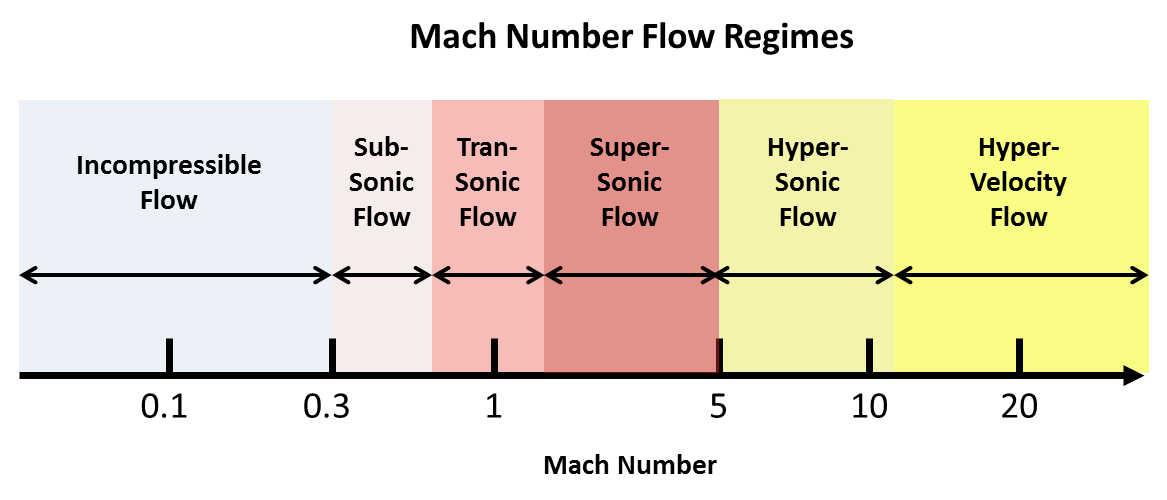
\includegraphics[width=10cm]{Mach-Number-Flow-Regimes}
    \caption{Mach-Number-Flow-Regimes}
\end{figure}

高马赫数流动必须考虑粘性耗散(Viscous dissipation)和压力功(pressure work),模拟高马赫数流动现象必须结合考虑动量和能量传递。在流动过程中热导率$ k $和粘度$ \mu $的变化\textbf{按理想气体}假设来计算。一般使用Sutherland's Law。

\begin{equation}
k = k_{ref}\left( \frac{T}{T_{k,ref}} \right)^{3/2}\frac{T_{k,ref}+S_k}{T+S_k}
\end{equation}

其中,$ k_{ref} $为参考条件下的热导率(\si{\watt\per\meter\per\kelvin}),$ T_{k,ref} $为参考条件下的温度(\si{\kelvin}),$ S_k $为Sutherland常数(\si{\kelvin},每种气体都有自己的常数)。

同理,高马赫流动流体的粘度也可使用Sutherland's Law来计算,\textbf{仅对低压下的单组分气体有效}。

\begin{equation}
\mu = \mu_{ref}\left( \frac{T}{T_{\mu,ref}} \right)^{3/2}\frac{T_{\mu,ref}+S_\mu}{T+S_\mu}
\end{equation}

其中,$ \mu_{ref} $为参考条件下的粘度(\si{\pascal\per\second}),$ T_{\mu,ref} $为参考条件下的温度(\si{\kelvin}),$ S_\mu $为Sutherland常数(\si{\kelvin},每种气体都有自己的常数)。

\section{多孔介质流动}

设多孔介质的基体体积为$ V_s $,孔隙的体积为$ V_f $,整个介质总体积为$ V_m = V_s + V_f $,多孔介质流道所占体积分数为孔隙率$ \varepsilon=V_f/V_m $。

多孔介质单位横截面积(包含孔隙和基体)的体积流率,即在$ V_m $上的平均流速称为\textbf{Darcy速度};在$ V_f $上的平均流速称为\textbf{内在平均速度(The intrinstic average velocity)或孔隙速度(pore velocity)}。

为了使孔隙速度$ u_p $有意义,必须对表征体元(包括孔隙体积和孔隙体积)上的速度进行统计平均,Darcy速度$ u_D $和孔隙速度$ u_p $可以通过Dupuit–Forchheimer relationship进行关联,这个定义使得速度在多孔区域和自由流动区域的边界上连续。

\begin{equation}\label{Dupuit–Forchheimer-relationship}
u_{D} = \varepsilon u_p
\end{equation}

运用通用的守恒方程导出多孔介质流动的连续性方程:

\begin{equation}
\varepsilon \frac{\partial \rho}{\partial t} + \nabla\cdot(\rho\bm{u}) = 0
\end{equation}

Darcy定律表明,流速和压力梯度成正比,流动的阻力主要是流体的粘性力,Darcy适用于低$ Re $的渗流情况。

\begin{equation}\label{Darcy's-law-2D}
u = -\frac{\kappa}{\mu} \frac{\partial p}{\partial x}
\end{equation}

三维情况下,Darcy定律如下式,其中$ \bm{\kappa} $为渗透率张量。

\begin{equation}\label{Darcy's-law-3D}
\bm{u} = -\frac{\bm{\kappa}}{\mu}\cdot\nabla p
\end{equation}

\subsection{渗透率}

流体流过固体基质的水力半径定义为:

\begin{equation}
d_h = \frac{4\times\text{void volume}}{\text{surface area}} = \frac{4\varepsilon}{A_0(1-\varepsilon)}
\end{equation}

其中,$ A_0 $是基于固体体积的比表面积,

\[A_0=\frac{A_{fs}}{V_s}\]

使用曲折因子对压力梯度进行修正,

\begin{equation}
\nabla p_{mod} = \frac{1}{\tau}\nabla p
\end{equation}

其中,曲折因子定义为流动的有效长度$ L_e $和流道进出口直线距离$ L $之比,

\[\tau = \frac{L_e}{L}\]

利用曲折因子$ \tau $和形状参数$ k_0 $来修正Hagen–Poiseuille equation推导的渗流速度,

\begin{equation}
\mathbf{u}_p = \frac{d_h^2}{16k_0\mu\tau}\nabla p
\end{equation}

其中,圆形毛细管的$ k_0=2 $,矩形毛细管的$ k_0=2.0\sim2.5 $,其他形状查阅文献\footnote{Johnson R W. Handbook of fluid dynamics [M]. Crc Press, 2016.}获知。

进一步可对孔隙速度与渗流速度的关联进行修正,

\begin{equation}
\mathbf{u}_D = \mathbf{u}_p\frac{\varepsilon}{\tau} = -\frac{\kappa}{\mu}\nabla p
\end{equation}

求解得到渗透率$ \kappa $,

\begin{equation}
\kappa = \frac{\varepsilon d_h^2}{16k_0\tau^2} =
\frac{\varepsilon d_h^2}{16k_\kappa} = 
\frac{\varepsilon^3}{k_\kappa (1-\varepsilon)^2A_0^2}
\end{equation}

其中,$ k_\kappa = k_0\tau^2 $称为Kozeny constant。

对于任意形状的颗粒,引入等效球体的概念,该颗粒与等效球体具有相同的比表面积,并定义等效球体直径为,

\begin{equation}
d = \frac{6}{A_0}
\end{equation}

对于尺寸均一、直径为$ d_s $的球形来说,$ d=d_s $;对于直径为$ d_c $的圆柱来说,$ d=(3/2)d_c $。

引入等效直径后,渗透率表示为,

\begin{equation}
\boxed{\kappa = \frac{\varepsilon^3}{36k_\kappa(1-\varepsilon)^2}d^2}
\end{equation}

渗透率是由多孔介质几何结构决定的,对于简单和规则的几何结构,我们能够通过几何参数来计算渗透率。比如球形颗粒填充床,渗透率与孔隙率、几何参数有如下关系:

\begin{equation}\label{Carman-Kozeny}
\kappa = \frac{d_p^2\varepsilon^3}{180(1-\varepsilon)^2}
\end{equation}

对于粒径分布较窄的球形填充床,文献提供的预测公式为,

\begin{equation}
\kappa = \frac{\varepsilon^5.5}{5.6}d^2
\end{equation}

\subsection{Forchheimer's Equation}

当Darcy流速$ \bm{u} $足够小(通常意味着$ Re<=1 $),流动符合Darcy定律。随着流速逐渐增大,惯性力带来的非线性曳力逐渐增强,在$ 1<=Re<=10 $这个范围内,惯性力的增长都比较平滑。一旦$ Re $足够高,流动的阻力将主要是流体与流道的摩擦力和惯性力。Forchheimer方程扩展了Darcy定律,适用于多孔介质内的快速流动。大量研究表明,从Darcy流动到Darcy–Forchheimer流动的转变发生在$ Re_{\text{local}}>100 $时。

\begin{equation}\label{Forchheimer}
\nabla p = -\frac{\mu}{\kappa}\bm{u} - c_F \kappa^{-1/2}\rho|\bm{u}|\bm{u}
\end{equation}

其中,$ c_F $为无量纲阻力系数,根据Beavers等人的实验总结,阻力系数可按下式计算:

\begin{equation}
c_F = 0.55 \left( 1-5.5\frac{d}{D_e} \right)
\end{equation}

其中,$ d $为颗粒直径,$ D_e $为床层等效直径,$ D_e=2wh/(w+h) $,$ w $为床层宽度,$ h $为床层高度。

除了Forchheimer方程外,Irmay等人也提出了一个关联多孔介质压降的关联式,当$ \beta=150 $,$ \alpha=1.75 $即为著名的Ergun方程:

\begin{equation}\label{Irmay}
\frac{dp}{dx}=-\frac{\beta\mu(1-\varepsilon)^2 u}{d_p^2\varepsilon^3}-\frac{\alpha\rho(1-\varepsilon)u^2}{d_p\varepsilon^3}
\end{equation}

\subsection{Brinkman's Equation}

\begin{equation}\label{Brinkman}
\rho\left[ \frac{1}{\varepsilon}\frac{\partial \bm{u}}{\partial t} + \frac{1}{\varepsilon}\nabla\left( \frac{\bm{u\cdot u}}{\varepsilon} \right) \right] = -\nabla p + \frac{\mu}{\varepsilon}\nabla^2\bm{u}-\frac{\mu}{\kappa}\bm{u}-\frac{c_F\rho}{\kappa^{1/2}}|\bm{u}|\bm{u}
\end{equation}

\subsection{填充床的孔隙率}
大量实验表明,填充床的孔隙率是一个阻尼振荡函数,从壁面处$ \varepsilon=1 $振荡变化到$ 5d_p $处接近稳定。可用经验公式描述孔隙率的变化:

\begin{equation}
\varepsilon=\varepsilon_{\infty}\left[ 1+C e^{\left(-N\frac{y}{d_p}\right)} \right]
\end{equation}

其中,$ y $是距壁面的距离;$ C $,$ N $是经验参数,实验表明$ C=1.4 $,$ \varepsilon_{\infty}=0.4 $时,$ N=5\ \text{or}\ 6 $。

由于壁面附近孔隙率最大,流动过程中流速也最大,这种现象称为“沟流现象”(channeling effect)。

\section{湍流}









    \chapter{Mass Transport}

\section{多组分质量传递基本概念}

对多组分流体混合物而言$ m=\sum m_i $,质量浓度(\si{\kilogram\per\meter\cubed})定义为:

\[\rho_i = \frac{m_i}{V} \]

混合物的密度即为全部物质的质量浓度之和:

\[\rho = \sum\rho_i \]

类似地,混合物的物质的量(\si{\mole})、质量分数($ \sum \omega_i = 1 $)、摩尔分数分别定义为:

\[ n_i=\frac{m_i}{M_i} \]
\[ \omega_i = \frac{m_i}{m} \]
\[ x_i = \frac{n_i}{n} \]

并且有如下转换关系:

\[\rho_i = \rho\omega_i = \rho\frac{M_i}{M}x_i \]

混合物的等效摩尔质量(\si{\kilogram\per\mole})定义为:

\[ M = \sum M_i x_i \]

如果气体混合物是理想气体,则满足:

\[ PV=nRT \]
\[ PV=mR_m T \]

其中$ R_m $是混合物气体参数,定义为:

\[ R_m = \frac{n}{m}R = \frac{R}{M} \]

气体$ i $的分压为$ P_i $,根据Dalton定律有:

\[ P=\sum P_i \]

\section{Mass diffusivity}
扩散系数分为三类,热扩散系数$ \alpha $、质量扩散系数$ D $、动量扩散系数$ \upsilon $,单位均为\si{\square\meter\per\second}。定义Schmidt数为$ Sc=\upsilon/D $,根据动力学理论,理想气体的$ Sc=1 $,故$ Sc $数其主要用来表征气体与理想气体的偏差(即表征气体的非理想性)。

浓度梯度引起分子扩散,通常化合物在空气中的扩散系数为在水中的扩散系数的1000倍左右。扩散系数的国际单位为\si{\square\meter\per\second}。对气体而言,根据动力学理论可知,气体的扩散系数与温度和压力相关,关系通常为$ f(T^n/p) $(通常$ n=3/2 $),气体的扩散系数通常随温度升高或压力下降而增大。实际上,由于气体的非理想性,$ n $通常要更大,例如水汽在空气中扩散,$ n=2.072(250\si{\kelvin}<T<459\si{\kelvin}) $。

\textbf{气体的二元扩散系数}常用Chapman–Enskog theory,其中,$ M $为分子质量(\si{\kilogram\per\mol}),$ p $为压力(\si{\pascal}),$ \sigma_{ij} $为平均碰撞直径(\si{\angstrom}),$ \Omega $是一个温度相关的碰撞积分:

\begin{equation}
D_{AB} = 2.695\times 10^{-3}\cdot \frac{\sqrt{T^3 (M_A+M_B)/(2000M_AM_B)}}{p\sigma_A\sigma_B\Omega_D}
\end{equation}

\textbf{液体的二元扩散系数}常用Wilke-Chang equation,其中$ \mu_B $为动力粘度(\si{\newton\second\per\square\meter}),$ V_A $为正常沸点下的分子体积(\si{\cubic\meter\per\mole}),$ \phi_B $为溶剂的无量纲关联系数,默认为1:

\begin{equation}
D_{AB} = 3.5\times 10^{-15} \frac{(\phi_B M_B)^{1/2} T}{\mu V_A^{0.6}}
\end{equation}

几个扩散系数的参照:

\begin{table}[!htb]
    \centering
    \caption{几个扩散系数参照\si{\square\meter\per\second}}
    \begin{tabular}{cccc}
        \toprule
        物质 & 在空气中1atm & 在水中 \\
        \midrule
        甲醇 & $ 1.5\times10^{-5} $ & $ 1.64\times10^{-9} $ \\
        乙醇 & $ 1.1499\times10^{-5} $ & $ 1.216895\times10^{-9} $ \\
        氧气 & $ 1.76\times10^{-5}(25\si{\degreeCelsius}) $ & - \\
        苯酚 & $ 8.2\times10^{-6} $ & $ 9.1\times10^{-10} $ \\
        \bottomrule
    \end{tabular}
\end{table}

上面两个公式是基于分子动力学,比较难用,主要是涉及分子动力学的常数比较难寻找。Fuller提出了一个气体扩散系数的经验关联式,形如$ D_{AB}=f(T^{1.75}/p) $,简单易用,误差不超过$ 10\% $。详情参见文献\cite{poling2001properties}。

\begin{equation}
D_AB=\frac{0.00143T^{1.75}}{pM_{AB}^{1/2}\left( \sum_{V_A}^{1/3} + \sum_{V_B}^{1/3} \right)^2 }
\end{equation}

其中$ D_{AB} $为二元扩散系数(\si{cm\squared\per\second});$ T $为温度(\si{\kelvin}),$ M_{AB}=2M_A M_B/(M_A + M_B) $;$ M_A $,$ M_B $为相对分子质量(\si{\g\per\mole});$ p $为压力(\si{bar})。

\section{Thermal Diffusion/Soret effect}

由温差引起的扩散称为\textbf{Soret效应},也称热泳(\url{https://en.wikipedia.org/wiki/Thermophoresis})。当混合物温差大、分子质量相差大时会产生热扩散,分子质量高的物质在低温区域积累,分子质量低的物质在高温处积累。多组分混合物所有热扩散系数之和为0:

\begin{equation}
\sum_{i=1}^Q D_i^T = 0
\end{equation}

\section{浓物质传递}
由$i$个物质构成的,有$j$个反应的反应流、浓物质系统的质量守恒方程为:

\begin{equation}
    \frac{\partial}{\partial t}(\rho\omega_i) + \nabla\cdot(\rho\omega_i\bm{u}) = -\nabla\cdot\bm{j}_i + R_i
\end{equation}

其中$\omega_i$表示$i$物质的质量分数,$\bm{j}_i$为质量通量(mass flux)源项,表示分子扩散、电场迁移、热扩散等引起的通量。

\subsection{Maxwell-Stefan Description}
\textbf{Maxwell-Stefan}是最详细的扩散模型,计算消耗最大,是一个扩散占主导的模型。多组分混合物中,相对于质量平均速度的质量通量可使用通用的Fick方程定义,总的扩散通量依赖于物质的浓度梯度、温度、压力和外部驱动力:

\begin{equation}
    \bm{j}_i = -\rho\omega_i\sum_{k=1}^{Q} \tilde{D}_{ik} \bm{d}_{k} - D_i^T\nabla\ln T
\end{equation}

$\tilde{D}_{ik}$是多组分Fick扩散系数,$D_i^T$是热扩散系数,$\bm{d}_k$是扩散驱动力。对理想气体而言,扩散驱动力可表示为:

\begin{equation}
    \bm{d}_k = \frac{1}{cR_gT} \left[ \nabla p_k-\omega_k\nabla p - \rho_k \bm{g}_k +\omega_k \sum_{l=1}^{Q} \rho_l \bm{g}_l \right]
\end{equation}

其中,$p_k$为气体分压,$\rho_k$为物质$k$的密度,$\bm{g}_k$为作用于物质$k$的外部作用力(例如电场)。

\subsection{Mixture-Averaged Approximation}
\textbf{Mixture-Averaged}模型假定分压和温度变化对多组分扩散的影响可以忽略,假定由分子扩散引起的质量通量符合Fick定律,则分子扩散通量正比于摩尔分数的梯度,定义为:

\begin{gather}
    \bm{j}_{md,i} = -\rho_i D_i^m \frac{\nabla x_i}{x_i} \\
    \bm{j}_{md,i} = -\left( \rho D_i^m \nabla \omega_i + \rho \omega_i D_i^m \frac{\nabla M}{M} \right) \\
    \rho_i = \rho\omega_i, x_i = \frac{\omega_i}{M_i} M
\end{gather}

其中,混合物平均扩散系数定义为:

\begin{equation}
    D_i^m = \frac{1-\omega_i}{\sum_{k\neq i}^N \frac{x_k}{D_{ik}}}
\end{equation}

\subsection{Fick's law}
\textbf{Fick's law}是一个通用的模型,通常用来描述分子扩散不占主导地位的系统,不需要多组分扩散系数,计算消耗最低。

\section{多组分扩散系数}
Maxwell-Stefan扩散系数$ D_{ik} $,Fick扩散系数$ D_w^F $,热扩散系数$ D_w^T $。

二元Fick扩散系数是对称的(symmetric),其和Maxwell-Stefan扩散系数$D_{ik}$可以相互转换。

\begin{equation}
    \tilde{D}_{ik} = \tilde{D}_{ki}
\end{equation}

\section{化学吸附}
化学吸附只能发生在固体表面的活性位点$ \sigma $上,定义被A覆盖的活性位点与总活性位点之比为吸附率,剩下的为空位率:

\begin{gather}
    \theta_A = \frac{\sigma_A}{\sigma} \\
    \theta_V = 1-\theta_A
\end{gather}

分子的吸附速率$ r_{ads} $与表面空位率和气体分压成正比,解吸率与表面占有率成正比:

\begin{gather}
    r_{ads} = k_{ads}p_A\theta_V \\
    r_{des} = k_{des}\theta_A
\end{gather}

达到吸附平衡时,表观速率$ r=r_{ads}-r_{des}=0 $,有:

\[k_{ads}p_A(1-\theta_A)=k_{des}\theta_A\]

令$ K_A=\frac{k_{ads}}{k_{des}} $,称为\textbf{吸附平衡常数},得\autoref{Langmuir},称为Langmuir吸附等温式:

\begin{equation}\label{Langmuir}
    \theta_A = \frac{K_Ap_A}{1+K_Ap_A}
\end{equation}

为了根据本体浓度$ c $和表面浓度$ cs $来建立传递和反应方程,执行以下代换,其中$ \Gamma_s $为表面得最大吸附浓度:

\[\theta_A = c_s/\Gamma_s\]
\[p_A=cRT\]

将得到下式,粗体为吸附和脱附反应速率常数。

\begin{gather}
    r_{ads} = \bm{\frac{k_{ads}RT}{\Gamma_s}}c(\Gamma_s-c_s)\\
    r_{des} = \bm{\frac{k_{des}}{\Gamma_s}}c_s
\end{gather}

对于表面来讲,涉及表面扩散、吸附脱附、表面反应,质量守恒为:

\begin{equation}
    \frac{\partial c_s}{\partial t}+\nabla\cdot(-D_s\nabla c_s) = r_{ads}-r_{des}=R
\end{equation}

本体溶液的质量守恒用经典的对流扩散方程描述:

\begin{equation}
    \frac{\partial c}{\partial t} + \nabla\cdot(-D\nabla c+\bm{u}c) = R
\end{equation}

\section{多孔介质质量传递}

对每一个组分应用质量守恒定律,并忽略源汇项,得出基于质量浓度的\textbf{单组分质量守恒方程}:

\begin{equation}
\frac{\partial \rho_i}{\partial t} + \nabla\cdot(\rho_i\bm{U_i}) = 0
\end{equation}

将方程中的质量浓度和内在平均速度汇总,得出全部组分的质量守恒方程:

\begin{equation}
\frac{\partial \rho}{\partial t} + \nabla\cdot(\sum\rho_i\bm{U_i}) = 0
\end{equation}

使用$ \bm{U}=\frac{1}{\rho}\sum\rho_i\bm{U_i} $表示质量平均速度,得出:

\begin{equation}
\frac{\partial \rho}{\partial t} + \nabla\cdot(\rho\bm{U}) = 0
\end{equation}

我们定义物质$ i $相对于质量平均速度的运动为扩散(diffusion),$ \bm{U_i}-\bm{U} $为扩散速度,则扩散通量为:

\begin{equation}
\bm{j_i} = \rho_i(\bm{U_i} - \bm{U})
\end{equation}

则,考虑对流-扩散的单组分质量守恒方程为:

\begin{equation}
\frac{\partial \rho_i}{\partial t} + \nabla\cdot(\rho_i\bm{U}) = -\nabla\cdot \bm{j_i}
\end{equation}

根据Fick定律,$ \bm{j_i} = -D\nabla\rho $,在上式两端同时乘上孔隙率$ \varepsilon $以考虑多孔介质内的质量传递:

\begin{equation}
\varepsilon\frac{\partial \rho_i}{\partial t} + \varepsilon\nabla\cdot(\rho_i\bm{U}) = \varepsilon\nabla\cdot(D\nabla \rho_i)
\end{equation}

运用Dupuit–Forchheimer relationship,考虑多孔介质内部的有效扩散系数,并将上式改写为关于摩尔浓度:

\begin{equation}
\varepsilon\frac{\partial c_i}{\partial t} + \varepsilon\nabla\cdot(c_i\bm{u}) = \varepsilon\nabla\cdot(D_{eff}\nabla c_i)
\end{equation}

\section{化学反应}

化学反应速率表达式一般为:

\begin{equation}
\frac{dc}{dt} = -kc^n
\end{equation}

反应速率常数常常于温度和和活化能相关,一般由Arrhenius relationship给出:

\begin{equation}
k = A \exp(-\frac{E}{RT})
\end{equation}

和温度相关的Arrhenius表达式一般为:

\begin{equation}
k = A \left( \frac{T}{T_{ref}} \right) \exp(-\frac{E}{RT})
\end{equation}


    \chapter{Thermodynamics}
强度量:与物质的量无关的物理量,压力$ p $,温度$ T $。

广延量:与物质的量\textbf{有关}的物理量,具有可加性,质量$ m $,容积$ V $,内能$ E $,焓$ H $,熵$ S $。

比参数:将广延量化为强度量,让其与物质的量无关,方便比较。

\section{能量传递基本概念和状态方程}

经典理想气体状态方程:
\begin{equation}
\label{idealGas}
pV=nRT
\end{equation}

从\autoref{idealGas}推导出\textbf{理想气体密度公式}:
\begin{equation}
\rho = \frac{Mp}{RT} = \frac{p}{R_s T}
\end{equation}

对理想气体而言,各物理性质是压力$ p $和温度$ T $的函数,如$ \rho(p,T) $、$ c_p(p,T) $、$ \mu(T) $、$ k(T) $。

比气体常数(Specific gas constant):
\begin{gather}
R_s = \frac{R}{M} \\
R_s = c_p - c_v
\end{gather}

定压比热容$ c_p $,令的$ 1\si{\kilogram} $物质的温度上升$ 1\si{\kelvin} $所需的能量,单位\si{\joule\per\kilogram\per\kelvin}。

比热容比(The ratio of specific thermal capacities),常见的双原子气体的$ \gamma=1.4 $,大多数液体的$ \gamma=1.1 $,水的$ \gamma=1.0 $。
\begin{equation}
\gamma = \frac{c_p}{c_v}
\end{equation}

热扩散系数(Thermal diffusivity, \si{\meter\squared\per\second}),其中$ k $为热导率( \si{\watt\per\meter\per\kelvin}),$ \rho $为密度( \si{\kilogram\per\cubic\meter}),$ c_p $为定压比热容(\si{\joule\per\kilogram\per\kelvin})。其用于评估材料导热能力相对于储热能力的大小,$ \alpha $越大,导热能力越强。

\begin{equation}
\alpha = \frac{k}{\rho c_p}
\end{equation}

焦耳:

\[1\si{\joule} = 1\si{\newton\meter} = \frac{\si{\kilogram\meter\squared}}{\si{\second\squared}} = 1\si{\watt\second} \]

\[1W = 1\si{\joule\per\second}\]

根据Fourier定律,产热速率$ Q $(\si{\watt}=\si{\joule\per\second})定义为:

\begin{equation}
Q = \propto A \frac{\partial T}{\partial x}
\end{equation}

对于材料属性稳定的材料而言,比例系数是恒定的,将其定义为热导率$ k $(\si{\watt\per\meter\per\kelvin})。负号是因为传热的方向与温度梯度相反:

\begin{equation}
Q = -k A \frac{\partial T}{\partial x}
\end{equation}

热通量定义为单位面积上的传热速率,$ q $(\si{\watt\per\meter\squared}=\si{\joule\per\meter\squared\second}):

\begin{equation}
q = \frac{Q}{A}
\end{equation}

很容易将方程扩展到三维:

\begin{equation}
q = -k\nabla T
\end{equation}

通常,我们希望知道物体的温度分布,即温度在介质中随位置是如何变化的。一旦知道了这种分布,就可以用Fourier定律计算介质中任何一点的导热通量。

考虑一个匀质的介质,其温度分布$ T(x,y,z) $使用Cartesian坐标表示,同时,假定介质是静止且不可压缩的。在介质中定义一个无限小的微元控制体,$ dxdydz $。由于物体是静止的,所以不考虑机械能和系统与环境的做功。一旦物体内存在温度梯度,就会发生热传导,如果已知热通量$ q_x $、$ q_y $、$ q_z $,通过Taylor级数展开可以获取相应面的对面的热通量:

\begin{gather}
q_{x+dx} = q_x + \frac{q_x}{x}dx \\
q_{y+dy} = q_y + \frac{q_y}{y}dy \\
q_{z+dz} = q_z + \frac{q_z}{z}dz
\end{gather}

\begin{figure}
    \centering
    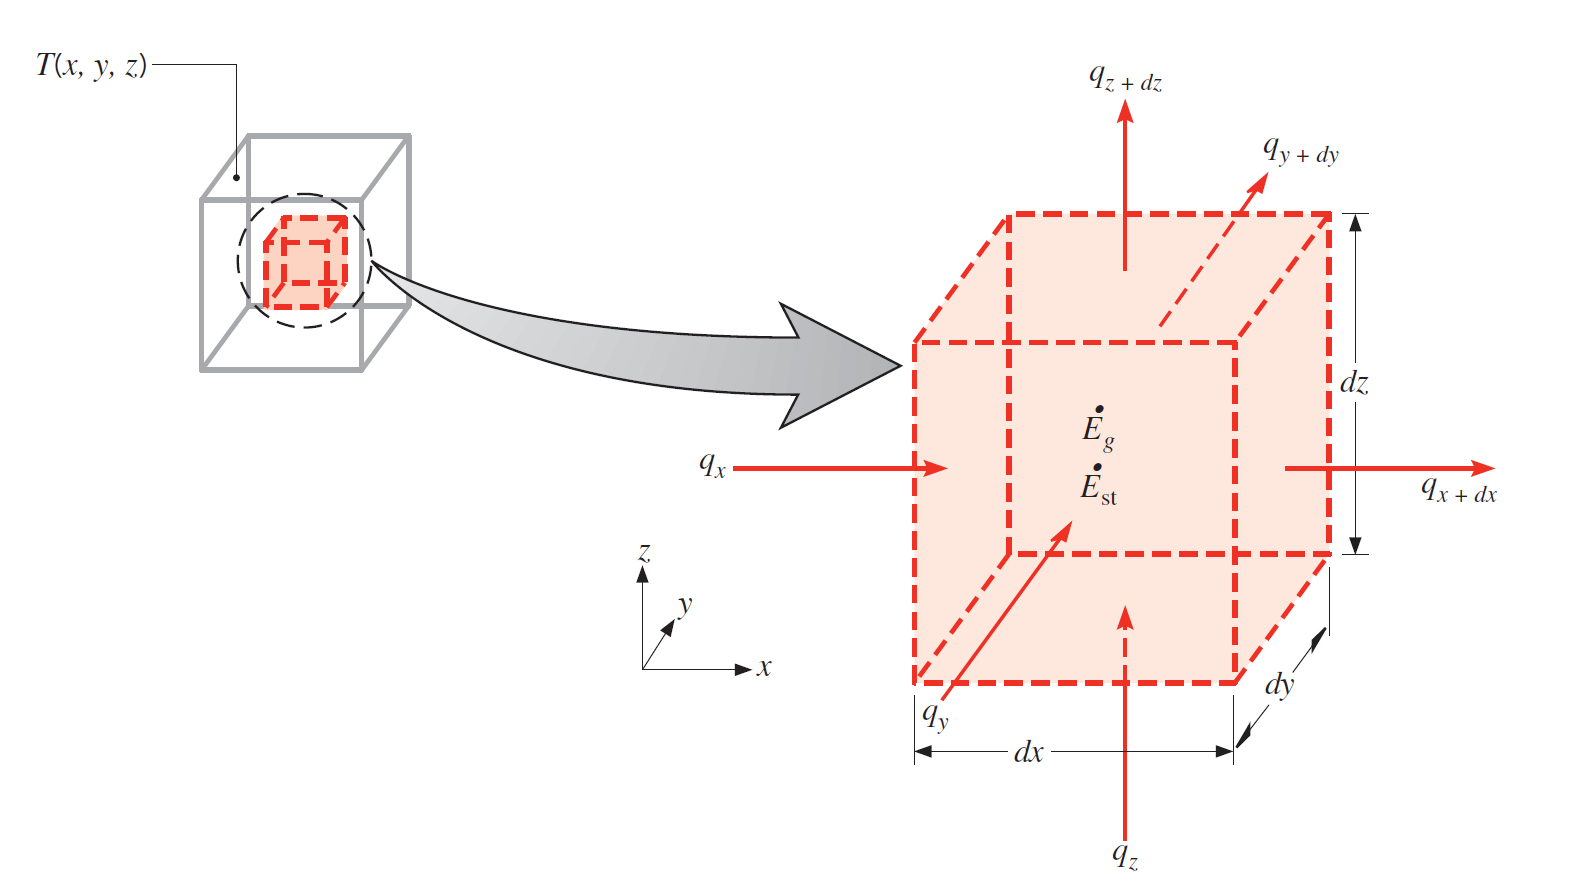
\includegraphics[width=12cm]{heat_conduction}
    \caption{Cartesian坐标系下的微元控制体}
\end{figure}

考虑介质中可能存在的能量源项,其中$ q_g $为单位体积的能力产生速率,(\si{\watt\per\meter\cubed}):

\begin{equation}
E_g = q_g dxdydz
\end{equation}

在介质不发生相变的情况下,不需要考虑潜热,所以介质内能量的变化率为显热(sensible energy)的变化率:

\begin{equation}
E_{cha} = \frac{\partial U_{sens}}{\partial t} = \rho c_v \frac{\partial T}{\partial t}dxdydz = \rho c_p \frac{\partial T}{\partial t}dxdydz
\end{equation}

其中,对不可压缩介质来说,定压比热容和定容比热容相等,$ c_v=c_p $。

将上述方程汇总,写出能量守恒的一般形式,

\begin{gather}
E_{in} - E_{out} + E_g = E_{cha} \\
q_x + q_y + q_z - q_{x+dx} - q_{y+dy} - q_{z+dz} + q_g dxdydz = \rho c_p \frac{\partial T}{\partial t} dxdydz \\
-\frac{\partial q_x}{\partial x} -\frac{\partial q_y}{\partial y} -\frac{\partial q_z}{\partial z} + q_g dxdydz = \rho c_p \frac{\partial T}{\partial t} dxdydz
\end{gather}

考虑材料性质为各向同性,根据Fourier定律来计算热通量:

\begin{gather}
q_x = -k dydz \frac{\partial T}{\partial x} \\
q_y = -k dxdz \frac{\partial T}{\partial y} \\
q_z = -k dxdy \frac{\partial T}{\partial z}
\end{gather}

将上述方程整合,并在两端除以控制体体积$ dxdydz $:

\begin{equation}
\frac{\partial}{\partial x}\left(k\frac{\partial T}{\partial x}\right) + \frac{\partial}{\partial y}\left(k\frac{\partial T}{\partial y}\right) + \frac{\partial}{\partial z}\left(k\frac{\partial T}{\partial z}\right) + q_g = \rho c_p \frac{\partial T}{\partial t}
\end{equation}

为了类比质量扩散方程,定义热扩散系数(thermal diffusivity)为$ \alpha = k/\rho c_p $:

\begin{equation}
\nabla^2 T + \frac{q_g}{k} = \frac{1}{\alpha} \frac{\partial T}{\partial t}
\end{equation}

\section{总能量方程}
能量守恒定义为绝热系统的总能量是一个常数。即总的能量不随时间变化,只能从一种形式转换为另一种形式且不能凭空消失。在CFD里面通常只考虑\textit{动能(机械能)}和\textit{分子内能(内能)}。能量守恒可以表示为:

\begin{center}
\textbf{流体微团内能量的变化率=流入的净热流量+体积力和表面力对微团做功的功率}
\end{center}

动能定义为:

\begin{equation}
K=\frac{1}{2}|\mathbf{u}|^2
\end{equation}

单位质量的内能定义为:$ E $,流体微团动能和内能总和的时间变化率定义为:

\begin{equation}
\rho\frac{D(K+E)}{Dt}dxdydz
\end{equation}

附加热源为$ Q $,流体微团的净热源为:

\begin{equation}
\rho Qdxdydz
\end{equation}

热通量为$ \bm{q}=-k\nabla T $,热传导对流体微团的加热为:

\begin{equation}
-\nabla \cdot\bm{q}dxdydz
\end{equation}

重力做功、压力和剪应力做功可以表示为:

\begin{gather}
\rho\bm{g}\cdot\bm{u}dxdydz \\
(-\nabla\cdot(p\bm{u}) + \nabla\cdot(\tau\cdot\bm{u})) dxdydz
\end{gather}

结合上式,总能量方程为(非守恒形式):

\begin{equation}
\rho\frac{D(K+E)}{Dt} =  -\nabla\cdot(p\bm{u}) + \rho Q - \nabla\cdot\bm{q} + \rho\bm{g}\cdot\bm{u} + \nabla\cdot(\tau\cdot\bm{u})
\end{equation}

总能量方程为(守恒形式):

\begin{equation}
\frac{\partial\rho E}{\partial t} + \frac{\partial\rho K}{\partial t} + \nabla\cdot(\rho\bm{u}E) + \nabla\cdot(\rho\bm{u}K) = -\nabla\cdot(p\bm{u}) + \rho Q - \nabla\cdot\bm{q} + \rho\bm{g}\cdot\bm{u} + \nabla\cdot(\tau\cdot\bm{u})
\end{equation}

\section{内能方程}

抽离动能项后我们能获取一个内能方程。首先,有动量守恒:

\begin{equation}
\rho \frac{D\mathbf{u}}{Dt} = \nabla\cdot\tau + \rho g + \nabla p
\end{equation}

将动量方程中的每个速度分量方程乘以速度分量并加和有:

\begin{equation}
\rho \frac{D \left[\dfrac{1}{2}\left(u_x^2+u_y^2+u_z^2 \right)= K\right]}{Dt}
=\left(\nabla \cdot \tau \right) \cdot \mathbf{u} + \rho \mathbf{g} \cdot \mathbf{u} -\mathbf{u} \cdot \nabla p
\end{equation}

与总能量方程相减得到内能方程:

\begin{equation}
\frac{DE}{Dt}
=-p\nabla \cdot \mathbf{u}-\nabla\cdot \mathbf{q} + \tau : \nabla \mathbf{u} + \rho Q
\end{equation}

\section{焓方程}

对于可压缩流体,通常我们把总能量方程简化为焓方程。定义比焓$ h $以及总比焓$ h_0 $:

\[ h = E+\frac{p}{\rho} \]
\[ h_0 = h+K \]

利用守恒形式的总能量方程可以得到\textit{守恒形式的比焓方程}和\textit{守恒形式的总比焓方程}:

\begin{equation}
\frac{\partial \rho h}{\partial t}+\nabla \cdot (\rho \mathbf{u} h) + \frac{\partial \rho K}{\partial t}+\nabla \cdot (\rho \mathbf{u} K) =\frac{\partial p}{\partial t}+ \rho Q - \nabla \cdot \mathbf{q} + \rho \mathbf{g} \cdot \mathbf{u}+\nabla \cdot(\tau \cdot \mathbf{u})
\end{equation}

\begin{equation}
\frac{\partial \rho h_0}{\partial t}+\nabla \cdot (\rho \mathbf{u} h_0) =\frac{\partial p}{\partial t}+ \rho Q - \nabla \cdot \mathbf{q} + \rho \mathbf{g} \cdot \mathbf{u}+\nabla \cdot(\tau \cdot \mathbf{u})
\end{equation}

在OpenFOAM的中,传热、可压缩、化学反应求解器求解的主要为\textit{守恒形式的总能量方程和比焓方程}。不可压缩流体常常忽略掉粘性应力耗散和重力做功项。

能量守恒相对于动量守恒要复杂一些。在不可压缩流动中,唯一重要的是内能方程。在考虑传热的情况下,内能要比热能小得多。只要温度对流体的影响不是很重要,那么能量方程可以放在压力速度耦合之后进行求解。在这种情况下是一种单向耦合。

需要注意,内能方程实际上来源于动量方程。但是总能量方程以及焓方程却可以单独推导。在某些情况下求解内能方程可能会带来一些问题。同时,对于不可压缩流体,能量的增加很少见,能量的耗散却比较明显。对于可压缩流,双方都比较重要。

\section{能量传递}

\subsection{能量守恒}
\textbf{热力学第一定理}表明,系统$\Omega$的动能$K_{\Omega}$、内能$E_{\Omega}$变化是由施加到系统上的机械能$P_{ext}$和热交换$Q_{exch}$引起的,动能$K_{\Omega}$、内能$E_{\Omega}$和压力(应力)$P_{str}$也有一定的转换关系,\textit{说明$P_{str}$通过耗散转化成了能量}。

\begin{gather}
    \frac{dE_{\Omega}}{dt} + \frac{dK_{\Omega}}{dt} = P_{ext} + Q_{exch} \\
    \frac{dK_{\Omega}}{dt} + P_{str} = P_{ext} \\
    \frac{dE_{\Omega}}{dt} = P_{str} + Q_{exch}
\end{gather}

系统$\Omega$的内能和内能的变化率定义如下:
\begin{gather}
    E_{\Omega} = \int_{\Omega} E dm \\
    \frac{E_{\Omega}}{dt} = \int_{\Omega} \frac{dE}{dt} dm = \int_{\Omega} \rho \frac{dE}{dt} dv
\end{gather}

连续介质假设推导出压力定义为:

\begin{equation}
    P_{str} = \int_{\Omega} (\bm{\sigma:D}) dv
\end{equation}

$\bm{\sigma}$和$\bm{D}$分别为应力张量和应变速率张量。操作符“:”的计算法则如下:

\begin{equation}
    \bm{a:b} = \sum_n \sum_m a_{nm}b_{nm}
\end{equation}

应力张量也可表示为$\sigma = -p\bm{I}+\tau$,所以$P_{str}$实际上是压力功(pressure-volume work)和粘性耗散(viscous
dissipation)之和:

\begin{equation}
    P_{str} = \int_{\Omega} p(\nabla\cdot \bm{u}) dv - \int_{\Omega}(\tau:\nabla \bm{u}) dv
\end{equation}

系统$\Omega$的热交换$Q_{exch}$是热传导、热辐射和附加热源引起的:

\begin{equation}
    Q_{exch} = - \int_{\partial\Omega} (\bm{q\cdot n}) ds - \int_{\partial\Omega} (\bm{q_r\cdot n}) ds + \int_{\Omega}Q dv
\end{equation}

热平衡方程表示如下:

\begin{equation}
    \int_{\Omega} \rho \frac{dE}{dt} dv + \int_{\partial\Omega} (\bm{q\cdot n}) ds + \int_{\partial\Omega} (\bm{q_r\cdot n}) ds = \int_{\Omega} (\bm{\sigma:D}) dv + \int_{\Omega} Q dv
\end{equation}

基本的传热是一个典型的\textbf{椭圆偏微分方程}:

\begin{gather}
    \rho C_p \frac{\partial T}{\partial t} + \nabla\cdot \bm{q} = Q \\
    \bm{q} = -k \nabla T
\end{gather}

施加Dirichlet或Neumann边界条件以求解:

\begin{gather}
    T = T_0\\
    -\bm{n\cdot q} = q_0
\end{gather}

当密度$\rho$,热容$C_p$,热导率$k$,热源$Q$,边界条件均为常数时,方程是一个线性系统。

\section{Boussinesq近似}

流体总是可压缩的,但如果密度变化对流动整体影响很小,但密度变化与流动有显著的耦合关系(如自然对流),可以只将密度的影响附加到体积力上,而忽略解密度对动量方程其他部分的影响。

流体的密度是压强和温度的函数,流体密度的相对变化可表示为:

\begin{equation}
\frac{\partial \rho}{\rho} = \frac{1}{\rho}\left(\frac{\partial \rho}{\partial p}\right)_T \delta p + \frac{1}{\rho}\left(\frac{\partial \rho}{\partial T}\right)_p \delta T
\end{equation}

方程右侧第一项的倒数称为体积弹性模量(\si{\newton\per\meter\squared}),

\[E_v = \rho\left(\frac{\partial p}{\partial \rho}\right)_T\]

热力学上,声速定义为,

\[a=\sqrt{\left(\frac{\partial p}{\partial \rho}\right)_s}\]

根据热力学定理,

\[\left(\frac{\partial p}{\partial \rho}\right)_s = \gamma \left(\frac{\partial p}{\partial \rho}\right)_T\]

对理想气体来说,$ p=\rho RT $,

\begin{equation}
a = \sqrt{\gamma RT}
\end{equation}

对液体和固体来说,$ \gamma = 1 $,于是有,

\begin{equation}
a=\sqrt{\frac{E_v}{\rho}}
\end{equation}



为了进行热对流,流体的密度必须时温度的函数$ \rho(T) $,因此我们需要一个状态方程来补充质量、动量、能量方程,密度状态方程为:

\begin{equation}
\rho_{\text{buoyancy}} = \rho_{ref}(1-\beta(T-T_{ref}))
\end{equation}

当流体受温度影响密度发生变化,但密度的变化非常小,且温度变化不足以介质的性质发生很大变化,可以使用Boussinesq近似来减小方程的非线性。Boussinesq假定在流动的控制方程中除了浮力项外,其他项的密度为是常数。

Boussinesq近似将流体看作不可压缩流体,即$ \nabla\cdot\bm{u} = 0 $,密度的变化仅影响体积力源项。其动量方程为:

\begin{equation}
\rho \frac{\partial \bm{u}}{\partial t} + \rho\nabla\cdot(\bm{uu}) = -\nabla p + \nabla\cdot(\mu\nabla\bm{u}) + \rho_{ref}(1-\beta(T-T_{ref}))\bm{g}
\end{equation}

\section{传热系数 The heat transfer coefficients}

当模拟因自然对流或强制对流产生的热量传递现象时,原则上采取两种方式:1.对表面应用传热系数,即假定与流体接触的边界上的对流热通量与热边界层上的温差成正比$-n\cdot q = h(T_{ext}-T)$;2.使用共轭传热(Conjugate Heat Transfer)或非等温流(Nonisothermal
Flow)直接计算模型与周围流体的热交换。

需要注意的是,如果计算了流体的对流现象,就不要使用换热系数。(It such case using heat transfer coefficients to model convective heat transfer is not relevant. Instead, modeling the fluid as immobile is likely to be accurate.)

通常根据对流的类型(自然或强制对流)和计算域的类型(外部或内部计算域)将对流传热分为四类。在自然对流中,有温差引起的浮力(buoyancy forces)起主要作用。传热系数$h$大多是通过经验和理论关联计算得出,首先定义一些无量纲数:

The Nusselt number, $Nu=hL/k$

The Reynolds number, $Re=\rho uL/\mu$

The Prandtl number, $Pr=\mu C_{p}/k$

The Rayleigh number, $Ra=GrPr$

其中$h$为换热系数(\si{\watt\per\square\meter\per\kelvin}),$k$为导热系数(\si{\watt\per\meter\per\kelvin})。

\section{多孔介质传热}
多孔介质传热涉及流-固两相,在不考虑非等温流动过程中的压力功和粘性耗散的情况下,各项能量传递控制方程写做。

固体总的能量传递:

\begin{equation}\label{solid-heat}
\rho_s C_{p,s} \frac{\partial T_s}{\partial t}+ \nabla\cdot\bm{q}_s = Q_s
\end{equation}

流体中的能量传递(忽略压力功和粘性耗散):

\begin{equation}\label{fluid-heat}
\rho_f C_{p,f} \frac{\partial T_f}{\partial t} + \rho_f C_{p,f}\bm{u}_f\cdot\nabla T_f + \nabla\cdot\bm{q}_f = Q_f
\end{equation}

流-固局部能量传递有\textbf{局部热平衡}和\textbf{非局部热平衡}两种假设。如果两相的吸热能力区别不大,大多数情况下可以假定两相温度相等。多porous plates(多孔板?)来讲,需要结合Sparrow number来判断局部热平衡假设是否还适用;对packed bed(填充床)来讲,需要结合Darcy number来判断。$ Sp<100 \text{or} 500 $,$ Da>10^{-7} $时,局部热平衡假设有效。

\begin{gather}
Sp = \frac{h_{sf}L^2}{k_{eff}r_h} \\
Da = \frac{\kappa}{d^2}
\end{gather}

其中$ h_{sf} $为流-固传热系数(\si{\watt\per\meter\squared\per\kelvin}),$ L $是平板厚度(\si{\meter}),$ k_{eff} $是多孔介质有效热导率(\si{\watt\per\meter\per\kelvin}),$ r_h $是水力半径(\si{\meter}),$ \kappa $是渗透率(\si{\square\meter}),$ d $是颗粒直径(\si{\meter})。

\subsection{多孔介质局部热平衡理论 Local Thermal Equilibrium}
局部热平衡假设流-固两相温度一致,即:

\[T_f=T_s=T\]

对\autoref{solid-heat}和\autoref{fluid-heat}所示的单相传热控制方程应用混合规则,固相能量传递乘上固相体积分数$ \theta_s $,流体相乘上流体体积分数$ 1-\theta_s $,多孔介质区域能量传递控制方程被整合为:

\begin{gather}
(\rho C_p)_{eff} \frac{\partial T_f}{\partial t} + \rho C_p\bm{u}\cdot\nabla T + \nabla\cdot\bm{q} = Q \\
\bm{q} = -k_{eff}\nabla T
\end{gather}

其中$ \rho $为流体密度,$ C_p $为流体定压热容,$ \bm{u} $是Darcy速度,即单位截面积的体积流率,平均线性速度(The average linear velocity,孔内的流速)$ \bm{u}_f=\bm{u}/(1-\theta_s) $。

$ (\rho C_p)_{eff} $为多孔介质体积有效定压热容:

\[(\rho C_p)_{eff} = \theta_s\rho_sC_{p,s} + (1-\theta_s)\rho_f C_{p,f}\]

$ k_{eff} $为有效热导率,取决于几何的复杂程度,有如下几种不同定义:

\begin{enumerate}
    \item 如果热传导在流-固两相同时发生,即两相没有净传热,则使用体积平均模型,按加权算术平均值计算
    \[k_{eff} =\theta_s k_s + (1-\theta_s)k_f\]
    \item 如果热传导按一定顺序依次在流-固两相发生,则使用加权调和平均值
    \[\frac{1}{k_{eff}} = \frac{\theta_s}{k_s} + \frac{1-\theta_s}{k_f} \]
    \item 按加权几何平均值来算
    \[k_{eff} = k_p^{\theta_s}\cdot k^(1-\theta_s) \]
\end{enumerate}

\subsection{多孔介质非等温流中的压力功和粘性耗散}

非等温流过程中,满足下式所示关系时,压力功效应可以被忽略:

\begin{equation}
\beta TL\left(\frac{g\beta}{c_{p,f}}\right) \ll 1
\end{equation}

当压力功效应不能被忽略时,需要向多孔介质的能量传递控制方程中添加压力功项:

\begin{equation}
(\rho C_p)_{eff} \frac{\partial T_f}{\partial t} + \rho C_p\bm{u}\cdot\nabla T + \nabla\cdot\bm{q} + \boxed{\beta T \left(\frac{\partial p}{\partial t}+\bm{u}\cdot\nabla p\right)} = Q
\end{equation}

同理,满足下式时,粘性耗散效应也可以被安全忽略:

\begin{equation}
L \left( \frac{g\beta}{c_{p,f}} \right) \ll 1
\end{equation}

Eckert Number也可以用来判断是否可以忽略压力功和粘性耗散,详情见\autoref{dimensionless-number}。粘性耗散常常写做:

\begin{equation}
\phi = \frac{\mu}{\kappa}\bm{u\cdot u} + \frac{c_p}{\kappa^{1/2}}|\bm{u}|\bm{u\cdot u} - \tilde{\mu}\bm{u}\cdot\nabla^2\bm{u}
\end{equation}

Nield等人进行了尺度分析,\textbf{将粘性耗散同热扩散项比较},提出了一个用于判别粘性耗散是否可被忽略的无量纲数。结果表明,当$ N\ll 1 $时,粘性耗散可被安全忽略。

\begin{equation}\label{Nield}
N = \frac{Br}{Da} = \frac{\mu U^2 L^2}{\kappa k_{eff}\Delta T}
\end{equation}

其涉及的无量纲数定义如下,其中$ Da $为Darcy number:

\[Br = \frac{Ec}{Pr} = \frac{\mu U^2}{k_{eff}\Delta T}\]

\[ Ec = \frac{U^2}{c_p \Delta T} \]

\[ Da = \frac{\kappa}{L^2} \]

对多孔介质内强制对流来讲,特征速度很好选择,且大多数情况下$ Da $数较小,也即在中等大小的Brinkman数下,粘性耗散的作用非常重要,不容忽视。

对自然对流来讲,特征速度$ U\approx (k_{eff}/\rho c_p L)Ra^{1/2} $,当$ Ge \ll 1 $时,可忽略自然对流过程中的粘性耗散,其中Gebhart number的定义为:

\[ Ge = \frac{g\beta L}{c_p} \]

上述的Nield数在P\'{e}clet数不太大的情况下能有效判别强制对流中的粘性耗散是否可以忽略,如果P\'{e}clet数过大,Nield数变为\textbf{粘性耗散和对流运输项之比}:

\[N = \frac{Ec}{DaRec}\]

\subsection{热分散 Thermal Dispersion}




    \chapter{实例}

整理几个上传一反的应用实例。

\section{固定床}

研究单个处于热流中的球形催化剂颗粒,如甲烷蒸汽重整或水汽变换。

\subsection{外扩散}

流体流过固体催化剂时,在固体表面会产生一个边界层。由于边界层内部速度几乎为0(壁面处等于0),所以穿过边界层到固体表面的质量传递是分子扩散引起的,这层边界层内的传递阻力也是流体向固体表面进行质量传递和能量传递的最大阻力。传质边界层$ \delta $一般定义为从固体表面到物质浓度达到流体主体浓度的99\%的距离,固体催化剂外表面的边界层传递阻力称为外扩散阻力。实际上,由于固体几何形貌的差异,流体流过固体时产生的边界层厚度不一致,造成固体表面的温度和浓度不均一。处理这些问题时,一般假设边界层厚度处处相等,这样可以将相间传递问题简化为一维问题,使复杂问题大大简化且能保持足够的精度。

由于流体速度越大,边界层厚度越小,所以其传递阻力主要由床层的水力学性能决定,除此之外,固体颗粒的几何性质、尺寸以及流体的物理属性等都会对传递阻力造成很大的影响。流体向固体表面的传质通量由传质系数和边界层两侧物理量的梯度来表示,传递系数反应了传递阻力的大小,传递阻力越大,传递系数越小。

\[ N=kA(c-c_s) \]

其中,$ N $为传质通量(\si{\mole\per\meter\cubed}),$ k $为传质系数(\si{\meter\per\second}),$ A $为固体的表面积(\si{\meter\squared})。

传质系数包含在Sherwood数中,定义为,

\[ Sh = \frac{hL}{D} = f(Re, Sc)\]

用$ j $因子关联气固传质和传热实验数据,传质和传热的$ j $因子分别定义为,

\[ j_m = \frac{h_m\rho}{G}Sc^{2/3}=\frac{h_m}{u}Sc^{2/3}=StSc^{2/3} \]

\[ j_h = \frac{h_h}{Gc_p}Pr^{2/3} =StPr^{2/3}\]


其中,传质系数$ h_m $(\si{\meter\per\second}),传热系数$ h_h $(\si{\watt\per\meter\squared\per\second})。传质系数将随着质量速度的增大而增大,即较高的流速加快了外扩散的传质速率,较低的流速会使外扩散阻力变大,甚至会成为过程的控制步骤。

将$ St $数的表达式带入$ j $因子表达式,得,

\[ Sh = j_m ReSc^{1/3} \]

\[ Nu = j_h RePr^{1/3} \]

传质关联由大量的实验数据得来,通常,对球形颗粒的传质关联为:

\[ Sh= 2+0.6Re^{1/2}Sc^{1/3} \]

球形颗粒的传热关联与传质关联形式完全一致,

\[ Nu=2+0.6Re^{1/2}Pr^{1/3} \]



\subsection{内扩散}

\subsection{多孔介质性质}

\subsection{1D homogeneous model}

\subsection{1D heterogeneous model}
    \chapter{Numerical Analysis}

\section{数值微分和数值积分}
当函数是初等函数时,可以使用\textbf{符号计算}求出其微积分,一旦函数是非初等函数,就只能使用\textbf{数值计算}方法了。

\subsection{Taylor's Formula}
首先看泰勒定理,其中$ c\in(x,x+h) $:
\begin{equation}
f(x) =f(x_0)+f'(x_0)(x-x_0) + \frac{f''(x_0)}{2!}(x-x_0)^2 +
\underbrace{\frac{f^{(n)}(c)}{n!}(x-x_0)^n}_{\text{remainder term}}
\end{equation}

\subsection{有限差分}
首先看导数的定义:

\begin{equation}
f'(x) = \lim_{h\rightarrow 0} \frac{f(x+h)-f(x)}{h}
\end{equation}

如果$ f $二阶连续可微,泰勒展开为:

\begin{equation}
f(x+h) = f(x)+hf'(x)+\frac{h^2}{2}f''(c)
\end{equation}

得出大名鼎鼎的\textbf{两点前向差分公式},其中$ c\in(x,x+h) $:

\begin{equation}
f'(x) = \frac{f(x+h)-f(x)}{h} - \frac{h}{2}f''(c)
\end{equation}

\section{Newton Cotes数值积分}
对定义在区间$ [a,b] $上的函数$ f $,可计算通过函数$ f(x) $的一些点的插值多项式的积分来近似$ f(x) $的积分。

梯形法则,其中$ h=x_1-x_0 $,$ c\in(x_0,x_1) $:

\begin{equation}
\int_{x_0}^{x_1}f(x)dx = \frac{h}{2}(y_0 + y_1) - \frac{h^3}{12}f''(c)
\end{equation}

辛普森法则,其中$ h=x_2-x_1=x_1-x_0 $,$ c\in(x_0,x_2) $:

\begin{equation}
\int_{x_0}^{x_1}f(x)dx = \frac{h}{3}(y_0 +4 y_1+y_2) - \frac{h^5}{12}f^{(4)}(c)
\end{equation}

\section{Gauss数值积分}

\begin{equation}
\int_1^1f(x)dx \approx \sum_{i=1}^n c_i f(x_i)
\end{equation}
    \backmatter
    \printbibliography[heading=bibliography,title=参考文献]
\end{document}